\section{Supplementary Figures}
%\section*{Figures}
% Supplementary
\renewcommand{\thefigure}{S\arabic{figure}}
\setcounter{figure}{0}
\begin{figure}[ht]
\centering
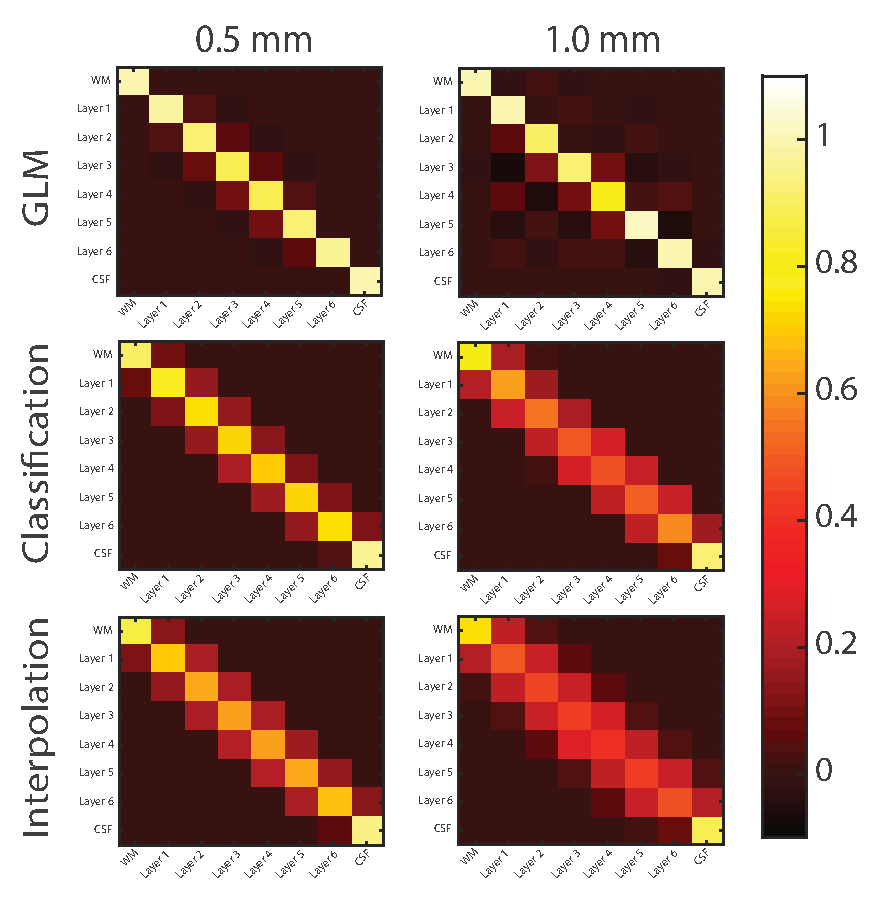
\includegraphics[width=0.9\textwidth, clip=true]{./Chapters/03_GLM/./Images/PointSpreadMatrices}
\caption{The point spread functions of all layers for both resolutions and both methods. An ideal point spread function would look like an identity matrix. This is approached more by the GLM method for both resolutions.}
\label{fig:pointspreadall}
\end{figure}